\newcommand{\defs}{../defs}
\documentclass[12pt,oneside,chapterprefix=true]{scrbook}

\usepackage[T1]{fontenc}
\usepackage[utf8x]{inputenc}
\usepackage[brazilian]{babel}
\usepackage[table]{xcolor}
\usepackage{minted}
\usepackage[a5paper,left=0.7cm,right=0.7cm,top=2cm,bottom=2.5cm,]{geometry}
\usepackage{url}
\usepackage{graphicx}
\usepackage[export]{adjustbox}
\usepackage{hyperref}
\usepackage[square]{natbib}
\usepackage[parfill]{parskip}
\usepackage{mdframed}
\usepackage{longtable}
\usepackage{soul}
\usepackage{tabularx}
\usepackage[shortlabels]{enumitem}
\usepackage{xifthen}
\usepackage{multirow}
\usepackage[portuguese, ruled, vlined, linesnumbered, algochapter]{algorithm2e}
\usepackage{amsmath}
\usepackage{amssymb}
\usepackage{amsthm}
\usepackage{tablefootnote}
\usepackage{subfigure}
\usepackage{gensymb}
\usepackage{pgfplots}
\usepackage{xpatch}
\usepackage{varwidth}
\usepackage[htt]{hyphenat}

\renewcommand{\familydefault}{\sfdefault}

\newcommand{\name}{Prof. Marcelo de Souza}
\newcommand{\email}{marcelo.desouza@udesc.br}
\newcommand{\course}{Bacharelado em Engenharia de Software}
\newcommand{\university}{Universidade do Estado de Santa Catarina}
\newcommand{\campus}{Centro de Educação Superior do Alto Vale do Itajaí}
\newcommand{\shortuniversity}{UDESC Ibirama}
\newcommand{\version}{Versão compilada em \today}
\newcommand{\exercisedescription}{Exercício}

\usepackage[automark,headsepline,footsepline]{scrlayer-scrpage}
\lehead{\content}
\lohead{\content}
\rehead{}
\rohead{}
\cehead{}
\cohead{}
\lefoot{\name}
\lofoot{\name}
\refoot{\\\thepage}
\rofoot{\\\thepage}
\cofoot{}
\cefoot{}
\setkomafont{pagehead}{\normalfont\small}
\setkomafont{pagefoot}{\normalfont}

\newpairofpagestyles{firstpage}{}

\newcommand{\makeheader}{
	\thispagestyle{firstpage}
	\vspace*{-42pt}
	\framebox[\textwidth]{
		\parbox{0.97\textwidth}{
			\begin{center}
				{\scriptsize\shortcourse\ -- \class}
				
				\vspace{10pt}
				
				\textbf{\content}
				
				\vspace{2pt}
				
				{\small\name}
				
				\vspace{10pt}
				
				{\scriptsize\shortuniversity\hfill\email}
				
				\vspace{-5pt}
				
				{\scriptsize\course\hfill\version}
				
			\end{center}
		}
	}
%	\vspace{-15pt}
%	\begin{flushright}
%		{\scriptsize\source}
%	\end{flushright}
	\smallskip
}

\renewcommand{\thesection}{\arabic{section}}

\allowdisplaybreaks

\hypersetup{
	colorlinks,
	linkcolor={blue!80!black},
	citecolor={blue!80!black},
	urlcolor={blue!80!black}
}

\definecolor{codelinecolor}{gray}{.90}
\colorlet{codeboxcolor}{blue!8}

\surroundwithmdframed{minted}

\BeforeBeginEnvironment{mdframed}{}
\AfterEndEnvironment{mdframed}{}

\mdfsetup{%
	backgroundcolor=codeboxcolor,
	linecolor=white}

\setminted{%
	mathescape,
	escapeinside=@@,
	linenos,
	breaklines,
	tabsize=3,
	fontsize=\footnotesize}

\newcommand{\code}[1]{%
	\sethlcolor{codelinecolor}
	\texttt{\hl{#1}}%
}

\newcommand{\inblock}[1]{%
	\sethlcolor{blockcolor}
	\hl{\mbox{#1}}%
}

\newcommand{\javacode}[1]{%
	\mintinline[escapeinside=~~]{java}{#1}
}

\newcommand{\javacodecolor}[1]{%
	\mintinline[escapeinside=~~,bgcolor=codeboxcolor]{java}{#1}
}

\newcounter{number}
\newenvironment{exercise}[1][]
{%
	\refstepcounter{number}%
	\noindent%
	\ifthenelse{\equal{#1}{}}%
		{\textbf{\exercisedescription~\thenumber.\\}}%
		{\textbf{\exercisedescription~\thenumber. (#1)\\}}%
	\rmfamily%
}{\medskip}%

\newcommand{\resetexercisenumbering}{
	\setcounter{number}{0}
}

\newcounter{solutionnumber}
\newenvironment{solution}[1][]
{%
	\refstepcounter{solutionnumber}%
	\noindent%
	\ifthenelse{\equal{#1}{}}%
	{\textbf{Solução -- \exercisedescription~\thesolutionnumber.\\}}%
	{\textbf{Solução -- \exercisedescription~\thesolutionnumber. (#1)\\}}%
	\rmfamily%
}{\medskip}%

\makeatletter%
\setlength{\@fptop}{5pt}

\def\arraystretch{1.5}

\newcommand{\insertspace}{\vspace{1.2em}}
\newcommand{\removespace}{\vspace{-1.2em}}

\setlength{\fboxsep}{0.8em}

\usepackage{array}
\newcolumntype{L}[1]{>{\raggedright\let\newline\\\arraybackslash\hspace{0pt}}m{#1}}
\newcolumntype{C}[1]{>{\centering\let\newline\\\arraybackslash\hspace{0pt}}m{#1}}
\newcolumntype{R}[1]{>{\raggedleft\let\newline\\\arraybackslash\hspace{0pt}}m{#1}}

\colorlet{blockcolor}{red!25}
\colorlet{redtext}{red!60!black}

\newcommand{\block}[1]{%
	\medskip
	\begin{figure}[H]
		\centering
		\begin{tikzpicture}
		\node [rectangle, align=center, fill=blockcolor, rounded corners=0.04cm, opacity = 1, text opacity = 1] {%
			#1
		};
		\end{tikzpicture}
	\end{figure}
}

\newcommand{\newtitle}[1]{%
	\begin{figure}[H]
		\begin{tikzpicture}
		\node [rectangle, fill=blue!30, rounded corners=0.04cm, opacity=1, text opacity=1, minimum width=\textwidth, text width=\linewidth-2*\pgfkeysvalueof{/pgf/inner xsep}, align=left] {%
			\textbf{#1}
		};
		\end{tikzpicture}
	\end{figure}
	\vspace{-10pt}
}

\renewcommand{\qedsymbol}{$\blacksquare$}
\xpatchcmd{\proof}{\itshape}{\normalfont\bfseries}{}{}

\newcommand{\content}{Estruturas de dados fundamentais}
\newcommand{\class}{Algoritmos e Estruturas de Dados}
\newcommand{\shortcourse}{45EST}

\begin{document}

\makeheader

{
Leitura obrigatória:
\begin{itemize}
	\item Capítulo 3 de~\cite{GoodrichEtAl2014} -- Estruturas de dados fundamentais.
\end{itemize}

Leitura complementar:
\begin{itemize}
	\item Capítulo 4 de~\cite{Preiss2001} -- Estruturas de dados fundamentais.
	\item Capítulo 2 de~\cite{Pereira2008} -- Listas lineares.
\end{itemize}
}

\medskip

\newtitle{Listas simplesmente encadeadas}

Problemas com o uso de arranjos:
\begin{itemize}
	\item Capacidade fixa.
	\item Inserção interna dificultada.
	\item Remoção interna dificultada.
\end{itemize}

\medskip

\textbf{Lista encadeada:} coleção de nodos formados em uma sequência linear.

\textbf{Lista simplesmente encadeada:} cada nodo armazena os dados do elemento e uma referência ao próximo nodo.

\begin{figure}[H]
	\centering
	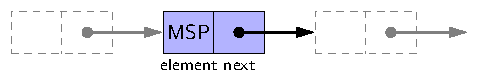
\includegraphics[width=0.7\linewidth]{img/figure-3-10}
\end{figure}

Elementos:
\begin{itemize}
	\item \texttt{head}: aponta para o primeiro elemento da lista.
	\item \texttt{tail}: aponta para o último elemento da lista.
	\item Último elemento aponta para \texttt{null}.
\end{itemize}

\begin{figure}[H]
	\centering
	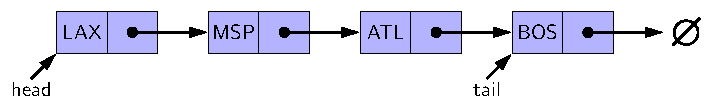
\includegraphics[width=0.9\linewidth]{img/figure-3-11}
\end{figure}

Benefícios:
\begin{itemize}
	\item Tamanho dinâmico.
	\item Consumo de memória dinâmico.
	\item Fácil inserção e remoção de elementos.
\end{itemize}

\bigskip

\textbf{Inserção de elemento no início}

\begin{figure}[H]
	\centering
	\setlength{\fboxsep}{0pt}
	\setlength{\fboxrule}{0pt}
	
	\framebox[0.7\textwidth][r]{
		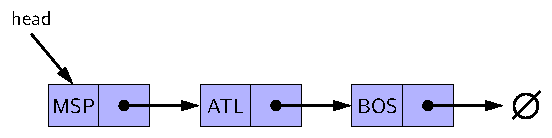
\includegraphics[width=0.54\linewidth]{img/figure-3-12a}
	}
	
	\framebox[0.7\textwidth][r]{
		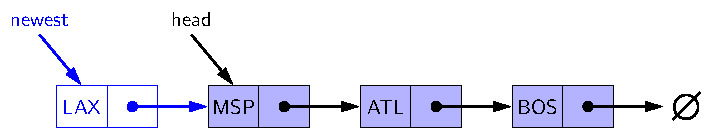
\includegraphics[width=0.7\linewidth]{img/figure-3-12b}
	}
	
	\framebox[0.7\textwidth][r]{
		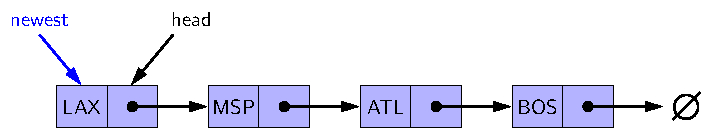
\includegraphics[width=0.7\linewidth]{img/figure-3-12c}
	}
\end{figure}

\textbf{Inserção de elemento no final}

\begin{figure}[H]
	\centering
	\setlength{\fboxsep}{0pt}
	\setlength{\fboxrule}{0pt}
	
	\framebox[0.7\textwidth][r]{
		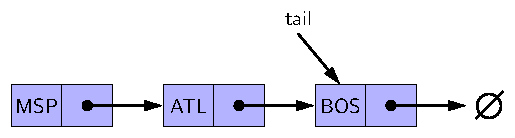
\includegraphics[width=0.48\linewidth]{img/figure-3-13a}
	}

	\framebox[0.7\textwidth][r]{
		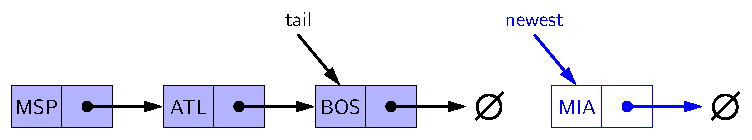
\includegraphics[width=0.7\linewidth]{img/figure-3-13b}
	}

	\framebox[0.7\textwidth][r]{
		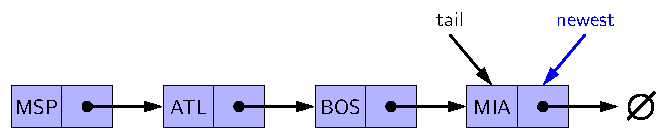
\includegraphics[width=0.62\linewidth]{img/figure-3-13c}
	}
\end{figure}


\textbf{Remoção de elemento}

\begin{figure}[H]
	\centering
	\setlength{\fboxsep}{0pt}
	\setlength{\fboxrule}{0pt}
	
	\framebox[0.7\textwidth][r]{
		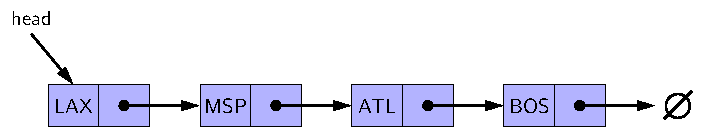
\includegraphics[width=0.7\linewidth]{img/figure-3-14a}	
	}
	
	\framebox[0.7\textwidth][r]{
		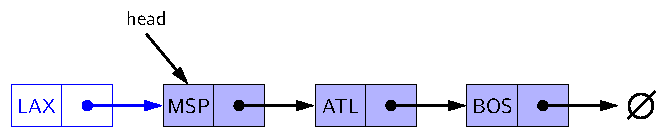
\includegraphics[width=0.7\linewidth]{img/figure-3-14b}
	}
	
	\framebox[0.7\textwidth][r]{
		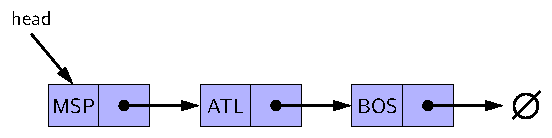
\includegraphics[width=0.55\linewidth]{img/figure-3-14c}
	}
\end{figure}

{\color{redtext}
Problemas na remoção do final:
\begin{itemize}
	\item Precisamos acessar o penúltimo elemento.
	\item Toda a lista tem que ser percorrida $\to$ custoso.
\end{itemize}
}

\textbf{Implementação}

\medskip

\begin{minted}{java}
public class SinglyLinkedList<E> {
	
	private static class Node<E> {
		private E element;
		private Node<E> next;
		
		public Node(E e, Node<E> n) {
			element = e;
			next = n;
		}
		
		public E getElement() { return element; }
		public Node<E> getNext() { return next; }
		public void setNext(Node<E> n) { next = n; }
	}
	
	private Node<E> head = null;
	private Node<E> tail = null;
	private int size = 0;
	
	public int size() { return size; }
	public boolean isEmpty() { return size == 0; }
	
	public E first() {
		if (isEmpty()) return null;
		return head.getElement();
	}
	
	public E last() {
		if (isEmpty()) return null;
		return tail.getElement();
	}
	
	// Métodos addFirst, addLast e removeFirst...
}
\end{minted}

\clearpage

{\color{redtext}
Comentários:
\begin{itemize}
	\item Classes externas não têm acesso à estrutura de nodos.
	\item Outros métodos podem ser implementados para manutenção da lista.
\end{itemize}
}

\bigskip

Método \texttt{addFirst(E e)}:
\begin{minted}{java}
public void addFirst(E e) {
	head = new Node<>(e, head);
	if (size == 0)
		tail = head;
	size++;
}
\end{minted}

\medskip

Método \texttt{addLast(E e)}:
\begin{minted}{java}
public void addLast(E e) {
	Node<E> newest = new Node<>(e, null);
	if (isEmpty())
		head = newest;
	else
		tail.setNext(newest);
	tail = newest;
	size++;
}
\end{minted}

\medskip

Método \texttt{removeFirst()}:
\begin{minted}{java}
public E removeFirst() {
	if (isEmpty()) return null;
	E answer = head.getElement();
	head = head.getNext();
	size--;
	if (size == 0)
		tail = null;
	return answer;
}
\end{minted}

\clearpage

\underline{Exercícios:}
\begin{enumerate}
	\item Implemente uma lista encadeada e use a estrutura para armazenar os dados dos alunos inscritos no SEMESO 2018 (nome, matrícula e fase). Crie métodos para inserção, remoção, consulta e listagem de inscritos.
\end{enumerate}

\bigskip

\newtitle{Listas encadeadas circulares}

Conceitos básicos:
\begin{itemize}
	\item Trata-se de uma lista encadeada com ordenação cíclica.
	\item Exemplos de uso:
	\begin{itemize}
		\item Jogadores de cartas.
		\item Escalonamento de processos.
	\end{itemize}
	\item ``Último'' elemento aponta para o ``primeiro''.
\end{itemize}

\begin{figure}[H]
	\centering
	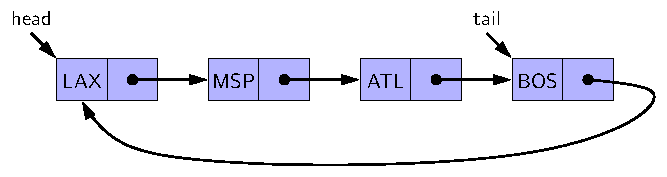
\includegraphics[width=0.7\linewidth]{img/figure-3-16}
\end{figure}

Novidades:
\begin{itemize}
	\item Não é necessária a referência para \texttt{head} (\texttt{tail.getNext()}).
	\item Novo método \texttt{rotate}, que atualiza a referência \texttt{tail}.
\end{itemize}

\clearpage

Método \texttt{rotate}:
\begin{figure}[H]
	\centering
	\begin{subfigure}
		\centering
		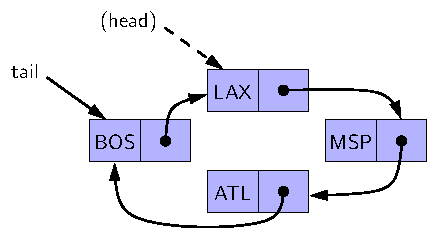
\includegraphics[width=.35\linewidth]{img/figure-3-17a}
	\end{subfigure}%
	\hspace{10pt}
	\begin{subfigure}
		\centering
		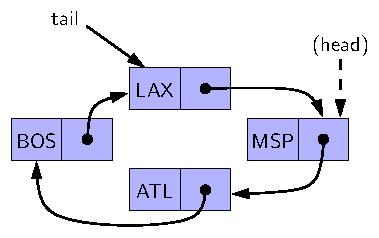
\includegraphics[width=.29\linewidth]{img/figure-3-17b}
	\end{subfigure}
\end{figure}

Método \texttt{addFirst}:
\begin{figure}[H]
	\centering
	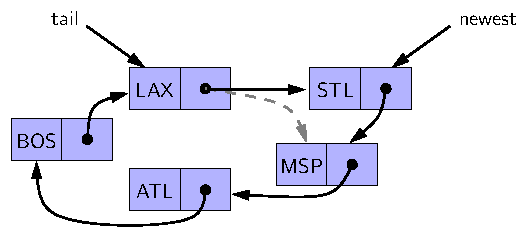
\includegraphics[width=0.5\linewidth]{img/figure-3-18}
\end{figure}

Método \texttt{addLast}:
\begin{itemize}
	\item Chama o método \texttt{addFirst} e atualiza a referência \texttt{tail}.
\end{itemize}
	
Método \texttt{removeFirst}:
\begin{itemize}
	\item Basta atualizar a referência \texttt{next} do elemento \texttt{tail}.
\end{itemize}

\clearpage

\textbf{Implementação}

\medskip

\begin{minted}{java}
public class CircularlyLinkedList<E> {
	
	//Definição da classe interna Node
	
	private Node<E> tail = null;
	private int size = 0;
	
	public int size() { return size; }
	public boolean isEmpty() { return size == 0; }
	
	public E first() {
		if (isEmpty()) return null;
		return tail.getNext().getElement();
	}
	
	public E last() {
		if (isEmpty()) return null;
		return tail.getElement();
	}
	
	public void rotate() {
		if (tail != null)
			tail = tail.getNext();
	}
	
	public void addFirst(E e) {
		if (size == 0) {
			tail = new Node<>(e, null);
			tail.setNext(tail);
		} else {
			Node<E> newest = new Node<>(e, tail.getNext());
			tail.setNext(newest);
		}
		size++;
	}

	public void addLast(E e) {
		addFirst(e);
		tail = tail.getNext();
	}

	public E removeFirst() {
		if (isEmpty()) return null;
		Node<E> head = tail.getNext();
		if (head == tail) tail = null;
		else tail.setNext(head.getNext());
		size--;
		return head.getElement();
	}

	public String toString() {
		if (tail == null) return "()";
		StringBuilder sb = new StringBuilder("(");
		Node<E> walk = tail;
		do {
			walk = walk.getNext();
			sb.append(walk.getElement());
			if (walk != tail)
				sb.append(", ");
		} while (walk != tail);
		sb.append(")");
		return sb.toString();
	}
}
\end{minted}

\medskip

\underline{Exercícios:}
\begin{enumerate}
	\item Implemente uma lista encadeada circular e use a estrutura para armazenar os dados dos jogos da Copa do Mundo 2018 (equipes, local e horário). Crie métodos para inserção, remoção, consulta e listagem de jogos.
\end{enumerate}

\clearpage

\newtitle{Listas duplamente encadeadas}

Problemas do encadeamento simples:
\begin{itemize}
	\item Deletar o último nodo. \inblock{$\gets$ como acessar o penúltimo elemento?}
	\item Deletar nodo tendo apenas sua referência?
\end{itemize}

\textbf{Lista duplamente encadeada:} cada nodo mantém a referência do \textit{anterior} (\texttt{prev}) e do \textit{próximo} (\texttt{next}) nodos.

\medskip

Sentinelas:
\begin{itemize}
	\item Nodos ``vazios'' usados para o início (\texttt{header}) e fim (\texttt{trailer}) da lista.
	\item Facilidade: certeza de que cada elemento possui dois vizinhos.
\end{itemize}

\begin{figure}[H]
	\centering
	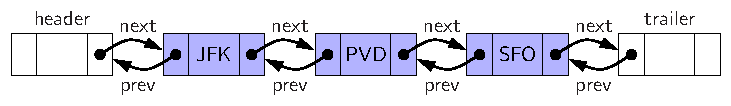
\includegraphics[width=0.8\linewidth]{img/figure-3-19}
\end{figure}

\textbf{Inserção de elemento no início}

\begin{figure}[H]
	\centering
	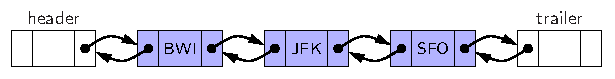
\includegraphics[width=0.58\linewidth]{img/figure-3-21a}
	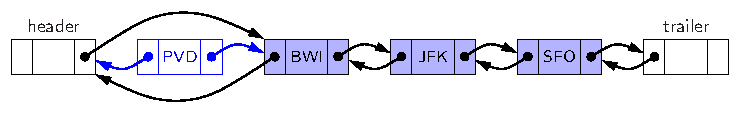
\includegraphics[width=0.7\linewidth]{img/figure-3-21b}
	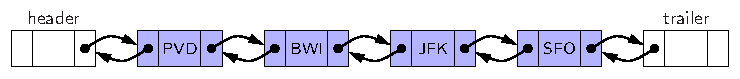
\includegraphics[width=0.7\linewidth]{img/figure-3-21c}
\end{figure}

\clearpage

\textbf{Inserção arbitrária de elemento}

\begin{figure}[H]
	\centering
	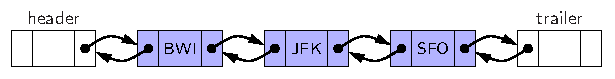
\includegraphics[width=0.58\linewidth]{img/figure-3-20a}
	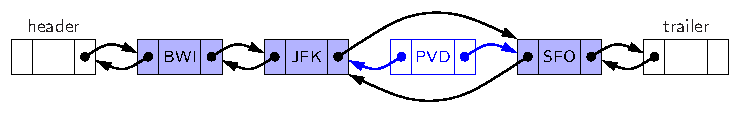
\includegraphics[width=0.7\linewidth]{img/figure-3-20b}
	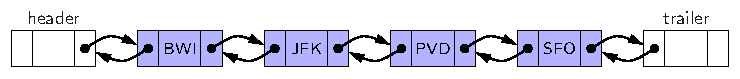
\includegraphics[width=0.7\linewidth]{img/figure-3-20c}
\end{figure}

\textbf{Remoção de elemento}

\begin{figure}[H]
	\centering
	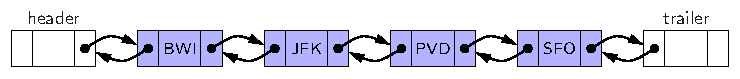
\includegraphics[width=0.7\linewidth]{img/figure-3-22a}
	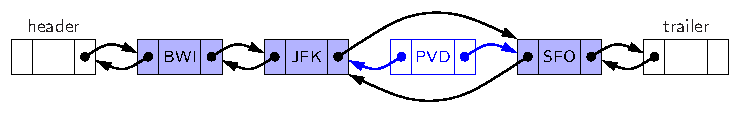
\includegraphics[width=0.7\linewidth]{img/figure-3-22b}
	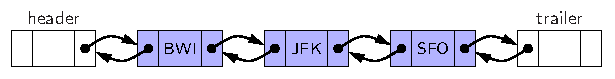
\includegraphics[width=0.58\linewidth]{img/figure-3-22c}
\end{figure}


\textbf{Implementação}

\medskip

\begin{minted}{java}
public class DoublyLinkedList<E> {
	
	private static class Node<E> {
		private E element;
		private Node<E> prev;
		private Node<E> next;
		
		public Node(E e, Node<E> p, Node<E> n) {
			element = e;
			prev = p;
			next = n;
		}
		
		public E getElement() { return element; }
		public Node<E> getPrev() { return prev; }
		public Node<E> getNext() { return next; }
		
		public void setPrev(Node<E> p) { prev = p; }
		public void setNext(Node<E> n) { next = n; }
	}
	
	private Node<E> header;
	private Node<E> trailer;
	private int size = 0;
	
	public DoublyLinkedList() {
		header = new Node<>(null, null, null);
		trailer = new Node<>(null, header, null);
		header.setNext(trailer);
	}
	
	public int size() { return size; }
	public boolean isEmpty() { return size == 0; }
	
	public E first() {
		if (isEmpty()) return null;
		return header.getNext().getElement();
	}
	
	public E last() {
		if (isEmpty()) return null;
		return trailer.getPrev().getElement();
	}
	
	public void addFirst(E e) {
		addBetween(e, header, header.getNext());
	}
	
	public void addLast(E e) {
		addBetween(e, trailer.getPrev(), trailer);
	}
	
	public E removeFirst() {
		if (isEmpty()) return null;
		return remove(header.getNext());
	}
	
	public E removeLast() {
		if (isEmpty()) return null;
		return remove(trailer.getPrev());
	}
	
	private void addBetween(E e, Node<E> pred, Node<E> succ) {
		Node<E> newest = new Node<>(e, pred, succ);
		pred.setNext(newest);
		succ.setPrev(newest);
		size++;
	}
	
	private E remove(Node<E> node) {
		Node<E> predecessor = node.getPrev();
		Node<E> successor = node.getNext();
		predecessor.setNext(successor);
		successor.setPrev(predecessor);
		size--;
		return node.getElement();
	}
	
	public String toString() {
		StringBuilder sb = new StringBuilder("(");
		Node<E> walk = header.getNext();
		while (walk != trailer) {
			sb.append(walk.getElement());
			walk = walk.getNext();
			if (walk != trailer)
			sb.append(", ");
		}
		sb.append(")");
		return sb.toString();
	}
}
\end{minted}

\medskip

\underline{Exercícios:}
\begin{enumerate}
	\item Implemente uma lista duplamente encadeada e use a estrutura para armazenar os dados dos pratos de um restaurante (nome e valor). Crie métodos para inserção, remoção, consulta e listagem de pratos.
\end{enumerate}

\medskip

\newtitle{Comparando estruturas de dados}

Ideia geral:
\begin{itemize}
	\item Comparação de objetos compara os ponteiros (espaço de memória).
	\item Sobrescrever o método \texttt{equals}, comparando os elementos.
	\item Cuidados: referência nula, classes distintas, tamanho da lista.
\end{itemize}

\medskip

Implementação:
\begin{minted}{java}
public boolean equals(Object o) {
	if (o == null) return false;
	if (getClass() != o.getClass()) return false;
	SinglyLinkedList other = (SinglyLinkedList) o;
	if (size != other.size) return false;
	Node walkA = head;
	Node walkB = other.head;
	while (walkA != null) {
		if (!walkA.getElement().equals(walkB.getElement()))
			return false;
		walkA = walkA.getNext();
		walkB = walkB.getNext();
	}
	return true;
}
\end{minted}

\medskip

\newtitle{Clonando estruturas de dados}

\underline{Importante:} na tentativa de copiar um objeto em Java, a cópia aponta para a mesma posição em memória (referência).
\begin{itemize}
	\item Solução: implementar a cópia no método \texttt{clone}.
\end{itemize}

\medskip

A estrutura de dados deve implementar a interface \texttt{Cloneable}:
\begin{minted}{java}
public class SinglyLinkedList<E> implements Cloneable {
\end{minted}

\medskip

O método \texttt{clone} deve ser sobrescrito:
\begin{itemize}
	\color{redtext}
	\item O programador decide o que manter a referência e o que copiar.
\end{itemize}

\bigskip

\begin{minted}{java}
public SinglyLinkedList<E> clone()
	    throws CloneNotSupportedException {
	    	
	SinglyLinkedList<E> other = (SinglyLinkedList<E>) super.clone();
	if (size > 0) {
		other.head = new Node<>(head.getElement(), null);
		Node<E> walk = head.getNext();
		Node<E> otherTail = other.head;
		while (walk != null) {
			Node<E> newest = new Node<>(walk.getElement(), null);
			otherTail.setNext(newest);
			otherTail = newest;
			walk = walk.getNext();
		}
	}
	return other;
}
\end{minted}

\clearpage

\newtitle{Atividades}

\begin{enumerate}
	\item Leia sobre as estratégias de geração de números aleatórios detalhadas em~\cite{GoodrichAndTamassia2013}.
	
	\item Faça os seguintes exercícios de reforço de~\cite{GoodrichEtAl2014}.
	\begin{itemize}
		\item[R-3.5:] O método \texttt{removeFirst} da classe \texttt{SinglyLinkedList} inclui um caso especial para redefinir o campo \texttt{tail} para \texttt{null} na remoção do último elemento da lista. Quais são as consequências de remover essas linhas de código? Explique por que a classe não funcionaria com esta modificação.
		
		\item[R-3.6:] Proponha um algoritmo para encontrar o penúltimo nodo em uma lista simplesmente encadeada na qual o último nodo possui uma referência nula no campo \texttt{next}.
		
		\item[R-3.7:] Considere o método \texttt{addFirst} da classe \texttt{CircularlyLinkedList}. O corpo do \texttt{else} depende de uma variável local \texttt{newest}. Projete um novo código para esta cláusula sem o uso de nenhuma variável local.
		
		\item[R-3.8:] Descreva um método para encontrar o nodo central de uma lista duplamente encadeada com nodos sentinelas, sem o uso de informações sobre o tamanho da lista. No caso de um número par de nodos, o método deve devolver o nodo à esquerda do ponto central. Qual a complexidade deste algoritmo?
		
		\item[R-3.9:] Forneça uma implementação para o método \texttt{size()} da classe \texttt{SinglyLinkedList}, considerando que a mesma não mantenha o tamanho armazenado em uma variável.
		
		\item[R-3.10:] Forneça uma implementação para o método \texttt{size()} da classe \texttt{CircularlyLinkedList}, considerando que a mesma não mantenha o tamanho armazenado em uma variável.
		
		\item[R-3.11:] Forneça uma implementação para o método \texttt{size()} da classe \texttt{DoublyLinkedList}, considerando que a mesma não mantenha o tamanho armazenado em uma variável.
		
		\item[R-3.15:] Implemente o método \texttt{equals()} para a classe \texttt{CircularlyLinkedList}, assumindo que duas listas são iguais se elas possuem a mesma sequência de elementos, com os elementos correspondentes no início da lista.
		
		\item[R-3.16:] Implemente o método \texttt{equals()} para a classe \texttt{DoublyLinkedList}. 
	\end{itemize}
	
	\bigskip
	
	\item Faça os seguintes exercícios de criatividade de~\cite{GoodrichEtAl2014}.
	\begin{itemize}
		\item[C-3.25:] Descreva um algoritmo para concatenar duas listas simplesmente encadeadas $L$ e $M$, em uma lista única $L'$ que contém todos os nodos de $L$ seguido de todos os nodos de $M$.
		
		\item[C-3.26:] Descreva um algoritmo para concatenar duas listas duplamente encadeadas $L$ e $M$ com sentinelas, em uma lista única $L'$.
		
		\item[C-3.27:] Descreva em detalhes como trocar dois nodos $x$ e $y$ de posição (não apenas seu conteúdo) em uma lista simplesmente encadeada $L$, dadas as referências para $x$ e $y$ somente. Repita este exercício para o caso em que $L$ é uma lista duplamente encadeada. Qual algoritmo possui maior complexidade?
		
		\item[C-3.28:] Descreva em detalhes um algoritmo para reverter uma lista simplesmente encadeada $L$ usando somente uma quantidade constante de espaço adicional.
		
		\item[C-3.31:] Nossa implementação de uma lista duplamente encadeada depende de dois nodos sentinelas, \texttt{header} e \texttt{trailer}, mas um único nodo sentinela para ambos início e fim seria suficiente. Reimplemente a classe \texttt{DoublyLinkedList} usando apenas um nodo sentinela.
	\end{itemize}
\end{enumerate}

\clearpage
\medskip

\newtitle{Referências}
\begingroup
	\footnotesize
	\renewcommand{\chapter}[2]{}%
	\bibliographystyle{apalike}
	\bibliography{../referencias}
\endgroup

\end{document}